% Fig. 10 -- Decision map in the (Drift, L) plane with the 30 labelled scenarios that carry Channel-B fields
% (single column, 3.5 in). Scenarios without a Tier-2 value are drawn at L = 1.
% Region boundaries are the iso-curves (1 - Drift) L = 0.50 and 0.85.
% Compile with pdfLaTeX (Overleaf default). Output: fig10_decision_map.pdf
\documentclass[border=3pt]{standalone}
\usepackage[T1]{fontenc}
\usepackage{newtxtext,newtxmath}
\usepackage{tikz}
\usepackage{pgfplots}
\pgfplotsset{compat=1.17}

\definecolor{acc}{RGB}{31,78,121}

\begin{document}
\footnotesize
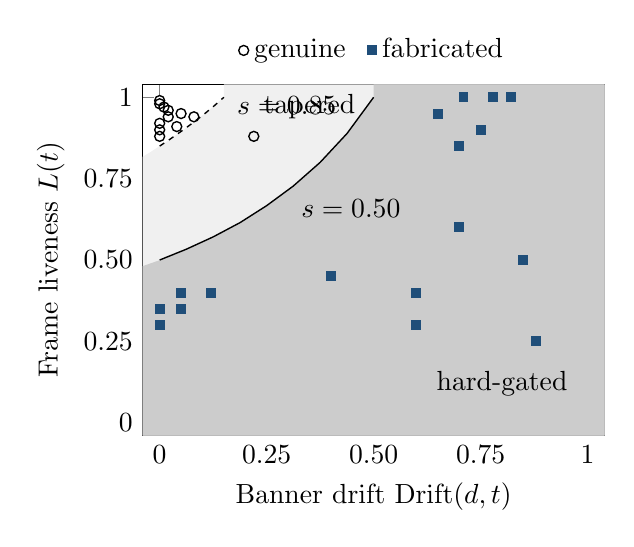
\begin{tikzpicture}
\begin{axis}[
    width=212pt, height=172pt,
    xmin=-0.04, xmax=1.04, ymin=-0.04, ymax=1.04,
    xtick={0,0.25,0.5,0.75,1}, xticklabels={0,0.25,0.50,0.75,1},
    ytick={0,0.25,0.5,0.75,1}, yticklabels={0,0.25,0.50,0.75,1},
    xlabel={Banner drift $\mathrm{Drift}(d,t)$},
    ylabel={Frame liveness $L(t)$},
    axis line style={line width=0.5pt}, tick style={line width=0.5pt},
    legend style={at={(0.5,1.03)},anchor=south,legend columns=2,draw=none,
                  /tikz/every even column/.append style={column sep=6pt}},
    clip=true,
]
  % tapered region: s < 0.85
  \addplot[fill=black!6,draw=none,forget plot] coordinates {
    (-0.040,-0.040) (1.040,-0.040) (1.040,1.040) (0.150,1.040) (0.150,1.000) (0.136,0.984) (0.123,0.969)
    (0.109,0.954) (0.096,0.940) (0.082,0.926) (0.069,0.913) (0.055,0.899) (0.041,0.887) (0.028,0.874)
    (0.014,0.862) (0.001,0.851) (-0.013,0.839) (-0.026,0.828) (-0.040,0.817)} -- cycle;
  % hard-gated region: s < 0.50
  \addplot[fill=black!20,draw=none,forget plot] coordinates {
    (-0.040,-0.040) (1.040,-0.040) (1.040,1.040) (0.500,1.040) (0.500,1.000) (0.461,0.928) (0.423,0.866)
    (0.384,0.812) (0.346,0.764) (0.307,0.722) (0.269,0.684) (0.230,0.649) (0.191,0.618) (0.153,0.590)
    (0.114,0.565) (0.076,0.541) (0.037,0.519) (-0.001,0.499) (-0.040,0.481)} -- cycle;

  % iso-curves
  \addplot[black,line width=0.5pt,forget plot] coordinates {
    (0.000,0.500) (0.062,0.533) (0.125,0.571) (0.188,0.615) (0.250,0.667) (0.312,0.727)
    (0.375,0.800) (0.438,0.889) (0.500,1.000)};
  \addplot[black,line width=0.5pt,dash pattern=on 2pt off 2pt,forget plot] coordinates {
    (0.000,0.850) (0.025,0.872) (0.050,0.895) (0.075,0.919) (0.100,0.944) (0.125,0.971) (0.150,1.000)};

  % genuine scenarios
  \addplot[only marks,mark=o,mark size=1.8pt,line width=0.5pt,mark options={fill=white,draw=black}] coordinates {
    (0.00,0.98) (0.05,0.95) (0.00,0.92) (0.02,0.96) (0.00,0.90) (0.04,0.91)
    (0.01,0.97) (0.00,0.88) (0.00,0.99) (0.02,0.94) (0.08,0.94) (0.22,0.88)};
  % fabricated scenarios
  \addplot[only marks,mark=square*,mark size=1.6pt,mark options={fill=acc,draw=acc}] coordinates {
    (0.75,0.90) (0.65,0.95) (0.00,0.35) (0.05,0.40) (0.70,0.85) (0.40,0.45) (0.60,0.40) (0.85,0.50)
    (0.00,0.30) (0.60,0.30) (0.82,1.00) (0.78,1.00) (0.71,1.00) (0.00,0.30) (0.05,0.35) (0.12,0.40)
    (0.88,0.25) (0.70,0.60)};
  \legend{genuine, fabricated}

  % curve and region labels
  \node[anchor=north west,inner sep=1.5pt] at (axis cs:0.32,0.70) {$s=0.50$};
  \node[anchor=west,inner sep=1.5pt] at (axis cs:0.17,0.975) {$s=0.85$};
  \node[anchor=center] at (axis cs:0.80,0.12) {hard-gated};
  \node[anchor=center] at (axis cs:0.35,0.97) {tapered};
\end{axis}
\end{tikzpicture}
\end{document}
